\documentclass[12pt]{article}
%\usepackage[utf8]{inputenc}
%\documentclass[UTF8]{ctexart}
%\usepackage[UTF8, heading = false, scheme = plain]{ctex}
\usepackage{geometry}
%geometry{a4paper,scale=0.9}
\geometry{a4paper,left=1cm,right=1cm,top=1cm,bottom=2cm}
\usepackage{amsfonts}
\usepackage{color}
\usepackage{url}
%\usepackage{biblatex}
\usepackage{amsmath}
\usepackage{amssymb}
\usepackage{latexsym}
\usepackage{cite}
%\addbibresource{ref.bib}
%\bibliography{ref.bib}
\usepackage{caption}
\usepackage{graphicx, subfig}
\usepackage{float}
%\usepackage[fontset=ubuntu]{ctex}
%\usepackage{fontspec}
\usepackage{xeCJK}
%\usepackage[colorlinks,
%anchorcolor=black,
%citecolor=black]{hyperref}
%\setmainfont{SimSun}
\usepackage[section]{placeins}
\usepackage{enumitem}
\usepackage{framed}
\usepackage[framemethod=TikZ]{mdframed}
\usepackage{indentfirst}
\usepackage{setspace}%使用间距宏包
\linespread{1.5}
%\title{预备知识}
%\author{leolinuxer }
%\date{June 2020}

\title{贝叶斯定理\cite{Fantastic_Bayesian_Common_Deduction}\cite{Common_Bayesian_Theory}\cite{Bayesian_Theory_With_Three_Examples}\cite{How_You_Understand_Bayesian}}
%\author{leolinuxer }
%\date{June 2020}

\begin{document}
%\setlength{\parindent}{0pt}
\maketitle
\tableofcontents

\section{相关背景}
\subsection{贝叶斯定理的产生来源}
英国数学家托马斯·贝叶斯(Thomas Bayes)在1763年发表的一篇论文中,首先提出了这个定理。而这篇论文是在他死后才由他的一位朋友发表出来的。在这篇论文中,他为了解决一个“\textbf{逆向概率}”问题,而提出了贝叶斯定理。

在贝叶斯写这篇文章之前,人们已经能够计算“\textbf{正向概率}”,比如杜蕾斯举办了一个抽奖,抽奖桶里有10个球,其中2个白球,8个黑球,抽到白球就算你中奖。你伸手进去随便摸出1颗球,摸出中奖球的概率是多大。根据频率概率的计算公式,你可以轻松的知道中奖的概率是2/10。

而贝叶斯在他的文章中是为了解决一个“逆概率”的问题。同样以抽奖为例,我们并不知道抽奖桶里有什么,而是摸出一个球,通过观察这个球的颜色,来预测这个桶里里白色球和黑色球的比例。

这个预测其实就可以用贝叶斯定理来做。贝叶斯当时的论文只是对“逆概率”这个问题的一个直接的求解尝试,这哥们当时并不清楚这里面这里面包含着的深刻思想。然而后来,贝叶斯定理席卷了概率论,并将应用延伸到各个问题领域。可以说,所有需要作出概率预测的地方都可以见到贝叶斯定理的影子,特别地,贝叶斯是机器学习的核心方法之一。

\subsection{为什么贝叶斯定理在现实生活中这么有用}
这是因为现实生活中的问题,大部分都是像上面的“\textbf{逆概率}”问题。生活中绝大多数决策面临的信息都是不完全的,我们手中只有有限的信息。既然无法得到全面的信息,我们就应该在信息有限的情况下,尽可能做出一个最优的预测。

比如,天气预报说,明天降雨的概率是30\%。这是什么意思呢?因为我们无法像计算\textbf{频率概率}那样,重复地把明天过上100次,然后计算出大约有30次会下雨,所以只能利用有限的信息(过去天气的测量数据),采用贝叶斯定理来预测出明天下雨的概率是多少。

同样的,在现实世界中,我们每个人都需要预测。要想深入分析未来、思考是否买股票、政策给自己带来哪些机遇、提出新产品构想,或者只是计划一周的饭菜。

贝叶斯定理就是为了解决这些问题而诞生的,它可以\textbf{根据过去的数据来预测出概率}。贝叶斯定理的思考方式为我们提供了明显有效的方法来帮助我们提供能力,以便更好地预测未来的商业、金融、以及日常生活。

也就是说,\textbf{在有限的信息下,贝叶斯定理,能够帮助我们预测出概率}。

\textbf{所有需要作出概率预测的地方都可以见到贝叶斯定理的影子},特别地,贝叶斯是机器学习的核心方法之一。例如垃圾邮件过滤,中文分词,艾滋病检查,肝癌检查等。

\section{数学形式}
\subsection{具体形式}
贝叶斯定理公式如下:
$$
P(A|B) = P(A) \frac{P(B|A)}{P(B)}
$$

各符号的含义如下:
\begin{itemize}
\setlength{\itemsep}{0pt}
\setlength{\parsep}{0pt}
\setlength{\parskip}{0pt}
    \item $A$:要求解的问题;
    \item $B$:已知信息;
    \item $P(A|B)$:后验概率;
    \item $P(A)$:先验概率
    \item $\frac{P(B|A)}{P(B)}$:可能性函数
\end{itemize}

\subsection{公式解读}
从公式来看,我们需要知道这么3个事情:

\textbf{1)先验概率}

我们把 $P(A)$ 称为"先验概率"(Prior probability),即在不知道 $B$ 事件发生的前提下,我们对 $A$ 事件发生概率的一个主观判断。

\textbf{2)可能性函数}

$P(B|A)/P(B)$称为"可能性函数"(Likelyhood),这是一个调整因子,即新信息事件 $B$ 的发生调整,作用是,使得先验概率更接近真实概率。

\textbf{可能性函数你可以理解为新信息过来后,对先验概率的一个调整}。比如我们刚开始看到“人工智能”这个信息,你有自己的理解(先验概率/主观判断),但是当你学习了一些数据分析,或者看了些这方面的书后(新的信息),然后你根据掌握的最新信息优化了自己之前的理解(可能性函数/调整因子),最后重新理解了“人工智能”这个信息(后验概率)
\begin{itemize}
\setlength{\itemsep}{0pt}
\setlength{\parsep}{0pt}
\setlength{\parskip}{0pt}
    \item 如果"可能性函数"$P(B|A)/P(B)>1$,意味着"先验概率"被增强,事件A的发生的可能性变大;

    \item 如果"可能性函数"=1,意味着B事件无助于判断事件A的可能性;

    \item 如果"可能性函数"<1,意味着"先验概率"被削弱,事件A的可能性变小。
\end{itemize}

\textbf{3)后验概率}

$P(A|B)$称为"后验概率"(Posterior probability),即在 $B$ 事件发生之后,我们对 $A$ 事件概率的重新评估。

现在我们再来看一遍贝叶斯公式,你现在就能明白这个公式背后的最关键思想了:\textbf{我们先根据以往的经验预估一个"先验概率"$P(A)$,然后加入新的信息(实验结果$B$),这样有了新的信息后,我们对事件$A$的预测就更加准确}。

因此,贝叶斯定理可以理解成下面的式子:

\textbf{后验概率(新信息出现后A发生的概率) = 先验概率(A发生的概率) x 可能性函数(新信息带出现来的调整)}

\textbf{贝叶斯的底层思想就是}:

如果我能掌握一个事情的全部信息,我当然能计算出一个客观概率(古典概率、正向概率)。
可是生活中绝大多数决策面临的信息都是不全的,我们手中只有有限的信息。既然无法得到全面的信息,我们就在信息有限的情况下,尽可能做出一个好的预测。也就是,在主观判断的基础上,可以先估计一个值(先验概率),然后根据观察的新信息不断修正(可能性函数)。

\subsection{\textbf{全概率公式}}
\textbf{这个公式的作用是计算贝叶斯定理中的$P(B)$}。

假定样本空间S,由两个事件A与A'组成的和。例如下图中,红色部分是事件A,绿色部分是事件A',它们共同构成了样本空间S。
\begin{figure}[H]
    \centering
    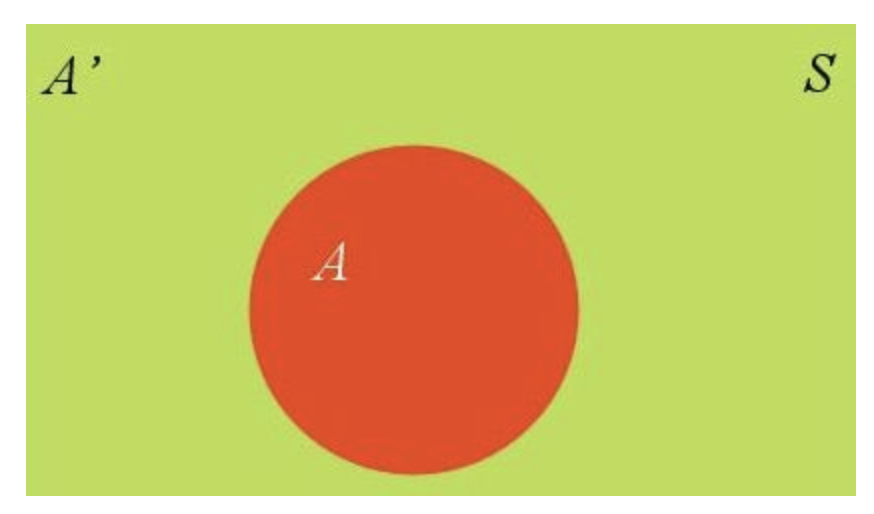
\includegraphics[width=.5\textwidth]{fig/Bayesian_Example_1.png}
\end{figure}

这时候来了个事件B,如下图:
\begin{figure}[H]
    \centering
    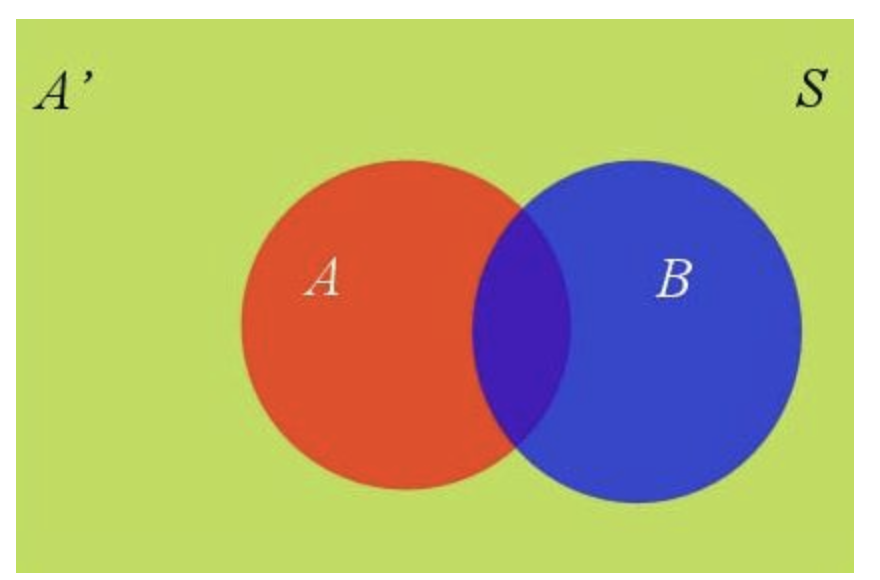
\includegraphics[width=.5\textwidth]{fig/Bayesian_Example_2.png}
\end{figure}

全概率公式:
$$
P(B) = P(B|A)P(A) + P(B|A')P(A')
$$

它的含义是,如果A和A'构成一个问题的全部(全部的样本空间),那么事件B的概率,就等于A和A'的概率分别乘以B对这两个事件的条件概率之和。

\section{连续形式下的贝叶斯公式}
\subsection{基本形式}
我们把上面例题中的 $A$ 变成样本(sample) $x$ , 把 $B$ 变成参数(parameter) $\theta$ , 便得到我们的贝叶斯公式:
$$
\pi(\theta_i|x) = \frac{f(x|\theta_i)\pi(\theta_i)}{\sum_if(x|\theta_i)\pi(\theta_i)}
$$

可以看出上面这个例子中,$B$ 事件的分布是离散的,所以在分母用的是求和符号。那如果我们的参数 $\theta$ 的分布是连续的呢?没错,那就要用积分,于是我们终于得到了真正的\textbf{贝叶斯公式} :
$$
\pi(\theta|x) = \frac{f(x|\theta)\pi(\theta)}{\int_\Theta f(x|\theta)\pi(\theta)d\theta}
$$

其中$\pi$指的是参数的概率分布,$\pi(\theta)$指的是先验概率,$\pi(\theta|x)$指的是后验概率,  $f(x|\theta)$指的是我们观测到的样本的分布,等价于似然函数(likelihood),记住\textbf{竖线 $|$ 左边的才是我们需要的}。其中积分求的区间$\Theta$指的是参数$\theta$所有可能取到的值的域,所以可以看出后验概率$\pi(\theta|x)$是在知道 $x$ 的前提下在$\Theta$域内的一个关于$\theta$的概率密度分布,每一个$\theta$都有一个对应的可能性(也就是概率)。

\subsection{进一步理解}
\subsubsection{似然函数}
首先来看似然函数 $f(x|\theta)$,似然函数听起来很陌生,其实就是我们在概率论当中看到的各种概率分布,那为什么后面要加个参数  $|\theta$ 呢?我们知道,掷硬币这个事件是服从伯努利分布的 $Ber(p)$ ,  $n$ 次的伯努利实验就是我们熟知的二项分布 $Bin(n,p)$ , 这里的 $p$ 就是一个参数,原来我们在做实验之前,这个参数就已经存在了(可以理解为上帝已经定好了),我们抽样出很多的样本  $x$ 是为了找出这个参数。以掷硬币为例,由于我们掷了1000次有492次是正面,根据求期望的公式 $n \cdot p = \mu$ (492就是我们的期望)可以得出参数 $p$ 为 $p = 492/1000 = 0.492$  ,所以我们可以认为正面的概率是近似50\%的。

现在我们知道了,其实我们观测到样本 $x$ 的分布是在以某个参数$\theta$ 为前提下得出来的,所以我们记为 $f(x|\theta)$ ,只是我们并不知道这个参数是多少。所以\textbf{参数估计}成为了统计学里很大的一个课题,古典统计学中常用的方法有两种:\textbf{矩方法(momnet)} 和\textbf{最大似然估计(maximum likelihood estimate, mle) },我们常用的像上面掷硬币例子中求均值的方法,本质就是矩估计方法,这是基于大数定理的。而统计学中更广泛的是使用最大似然估计的方法,原理其实很简单,在这简单说一下:假设我们有个$n$样本 $x_1, x_2, \cdots, x_n$, 它们每一个变量都对应一个似然函数:
$$
f(x_1|\theta), f(x_2|\theta), \cdots, f(x_n|\theta)
$$

我们现在把这些似然函数乘起来:
$$
like(\theta) = \prod_{i=1}^nf(x_i|\theta)
$$

我们只要找到令$like(\theta)$这个函数最大的 $\theta$ 值,便是我们想要的参数值。

\subsubsection{后验分布(Posterior distribution)}
现在到了贝叶斯的时间了。以前我们想知道一个参数,要通过大量的观测值才能得出,而且是只能得出一个参数值。而现在运用了贝叶斯统计思想,这个后验概率分布$\pi(\theta|x)$其实是一系列参数值$\theta$的概率分布,再说简单点就是我们得到了许多个参数$\theta$及其对应的可能性,我们只需要从中选取我们想要的值就可以了:
\begin{itemize}
\setlength{\itemsep}{0pt}
\setlength{\parsep}{0pt}
\setlength{\parskip}{0pt}
    \item 有时我们想要概率最大的那个参数,那这就是\textbf{后验众数估计(posterior mode estimator)};
    \item 有时我们想知道参数分布的中位数,那这就是\textbf{后验中位数估计(posterior median estimator)};
    \item 有时我们想知道的是这个参数分布的均值,那就是\textbf{后验期望估计}。
\end{itemize}

这三种估计没有谁好谁坏,只是提供了三种方法得出参数,看需要来选择。现在这样看来得到的参数是不是更具有说服力。

\subsubsection{置信区间和可信区间}
在这里我想提一下\textbf{置信区间(confidence interval, CI)}和\textbf{可信区间(credibility interval,CI)},我觉得这是刚学贝叶斯时候非常容易弄混的概念。

再举个例子:一个班级男生的身高可能服从某种正态分布 $N(\mu, \sigma^2)$ ,然后我们把全班男生的身高给记录下来,用高中就学过的求均值和方差的公式就可以算出来这两个参数,要知道我们真正想知道的是这个参数 $\mu, \sigma^2$,当然样本越多,得出的结果就接近真实值(其实并没有人知道什么是真实值,可能只有上帝知道)。等我们算出了均值和方差,我们这时候一般会构建一个95\%或者90\%的置信区间,这个置信区间是对于\textbf{样本}$x$来说的,我只算出了一个$\mu$和一个$\sigma$参数值的情况下,95\%的置信区间意味着在这个区间里的样本是可以相信是服从以$\mu, \sigma^2$为参数的正态分布的,一定要记住\textbf{置信区间}的概念中是指\textbf{一个参数值}的情况下!

而我们也会对我们得到的后验概率分布构造一个90\%或95\%的区间,称之为\textbf{可信区间}。这个可信区间是对于\textbf{参数}$\theta$来说的,我们的到了\textbf{很多的参数值},取其中概率更大一些的90\%或95\%,便成了可信区间。

\subsubsection{先验分布(Prior distribution)}
说完了后验分布,现在就来说说先验分布。先验分布就是你在取得实验观测值以前对一个参数概率分布的\textbf{主观判断},这也就是为什么贝叶斯统计学一直不被认可的原因,统计学或者数学都是客观的,怎么能加入主观因素呢?但事实证明这样的效果会非常好!

再拿掷硬币的例子来看,在扔之前你会有判断正面的概率是50\%,这就是所谓的先验概率,但如果是在打赌,为了让自己的描述准确点,我们可能会说正面的概率为0.5的可能性最大,0.45的几率小点,0.4的几率再小点,0.1的几率几乎没有等等,这就形成了一个先验概率分布。

那么现在又有新的问题了,如果我告诉你这个硬币的材质是不均匀的,那正面的可能性是多少呢?这就让人犯糊涂了,我们想有主观判断也无从下手,于是我们就想说那就先认为0~1之间每一种的可能性都是相同的吧,也就是设置成0~1之间的均匀分布$Uni(0,1)$作为先验分布吧,这就是贝叶斯统计学当中的\textbf{无信息先验(noninformative prior)}!那么下面我们就通过不断掷硬币来看看,这个概率到是多少,贝叶斯过程如下:
\begin{figure}[H]
    \centering
    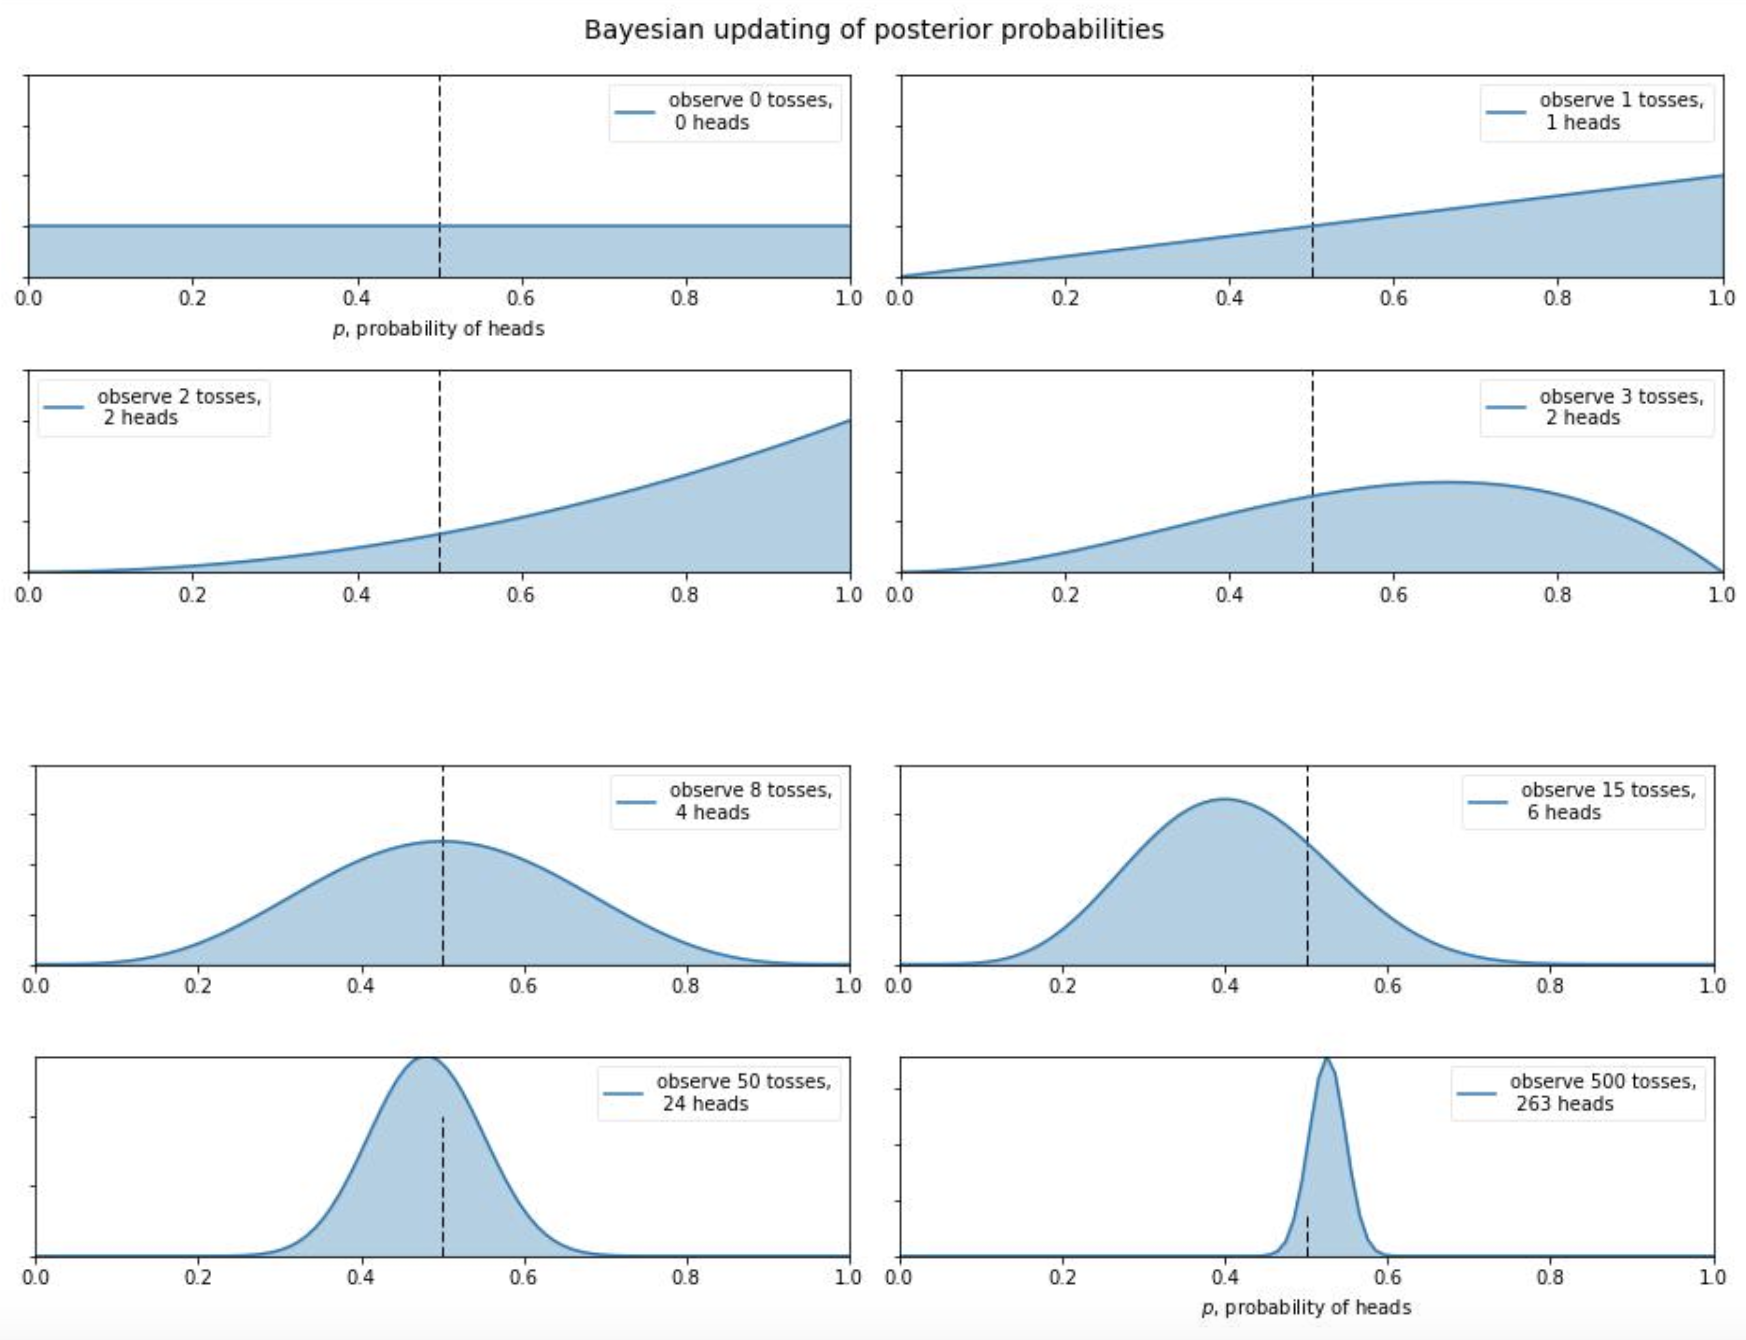
\includegraphics[width=1\textwidth]{fig/Bayesian_Example_4.png}
\end{figure}

作者:Yankun
链接:https://www.zhihu.com/question/21134457/answer/169523403
来源:知乎
著作权归作者所有。商业转载请联系作者获得授权,非商业转载请注明出处。

从图中我们可以看出,0次试验的时候就是我们的先验假设——均匀分布,然后掷了第一次是正面,于是概率分布倾向于1,第二次又是正,概率是1的可能性更大了,但\textbf{注意:这时候在0.5的概率还是有的,只不过概率很小,在0.2的概率变得更小}。第三次是反面,于是概率分布被修正了一下,从为1的概率最大变成了2/3左右最大(3次试验,2次正1次反当然概率是2/3的概率最大)。再下面就是进行更多次的试验,\textbf{后验概率不断根据观测值在改变},当次数很大的时候,结果趋向于0.5(哈哈,结果这还是一枚普通的硬币,不过这个事件告诉我们,直觉是不可靠的,一定亲自实验才行~)。有的人会说,这还不是在大量数据下得到了正面概率为0.5嘛,有什么好稀奇的?

\textbf{注意了}!我们上面就说到了古典概率学的弊端就是如果掷了2次都是正面,那我们就会认为正面的概率是1,而在贝叶斯统计学中,如果我们掷了2次都是正面,只能说明正面是1的可能性最大,但还是有可能为0.5, 0.6, 0.7等等的,这就是对古典统计学的一种完善和补充,于是我们也就是解释了,我们所谓的地震的概率为5\%;生病的概率为10\%等等这些概率的意义了,这就是贝叶斯统计学的哲学思想。

\subsubsection{共轭先验(Conjugate prior)}
共轭先验应该是每一个贝叶斯统计初学者最头疼的问题,我觉得没有“之一”。这是一个非常大的理论体系,我试着用一些简单的语言进行描述,关键是去理解其思想。

继续拿掷硬币的例子,这是一个二项试验 $Bin(n,p)$,所以其似然函数为:
$$
f(x|\theta) = \begin{pmatrix}n\\x\end{pmatrix}\theta^x(1-\theta)^{n-x}
$$

在我们不知道情况时就先假设其先验分布为均匀分布$Uni(0,1)$ ,即:
$$
\pi(\theta) = 1, \theta \in (0, 1)
$$

那现在根据贝叶斯公式求后验概率分布:
$$
\pi(\theta|x) = \frac{\theta^x(1-\theta)^{n-x}}{\int_0^1\theta^x(1-\theta)^{n-x}d\theta}
$$

我们得到结果为:
$$
\pi(\theta|x) = \frac{\Gamma(n+2)}{\Gamma(x+1)\Gamma(n-x+1)}\theta^{(x+1)-1}(1-\theta)^{(n-x+1)-1}
$$

这么一大串是什么呢?其实就是大名鼎鼎的贝塔分布(Beta distribution)。 简写就是 $Be(x+1, n-x+1)$。比如我掷了10次(n=10),5次正(x=5),5次反,那么结果就是$Be(6,6)$, 这个分布的均值就是0.5( $\frac{6}{6+6}$ ),很符合我们想要的结果。

现在可以说明,我们把主观揣测的先验概率定为均匀分布是合理的,因为我们在对一件事物没有了解的时候,先认为每种可能性都一样是非常说得通的。有人会认为,既然无信息先验是说得通的,而且贝叶斯公式会根据我们的观测值不断更新后验概率,那是不是我们随便给一个先验概率都可以呢?当然......不行!!这个先验概率是不能瞎猜的,是需要根据一些前人的经验和常识来判断的。比如我随便猜先验为一个分段函数:
$$
\pi(\theta) = \begin{cases}
1 \qquad if \ \theta \in (0, 0.2), (0.3, 0.5), (0.7, 1) \\
0 \qquad if \ \theta \in (0.2, 0.3), (0.5, 0.7) \\
\end{cases}
$$

就是假设一个极端的情况,如果你把这个情况代入贝叶斯公式,结果是不会好的(当然我也不知道该怎么计算)。

这个例子中,我看到了可能的后验分布是 $Beta$ 分布,看起来感觉有点像正态分布啊,那我们用正态分布作为先验分布可以吗?这个是可以的(所以要学会观察)。可如果我们把先验分布为正态分布代入到贝叶斯公式,那计算会非常非常麻烦,虽然结果可能是合理的。那怎么办?不用担心,因为我们有共轭先验分布!

继续拿上面这个例子,如果我们把先验分布$\pi(\theta)$设为贝塔分布 $Beta(a,b)$ ,结果是什么呢?我就不写具体的计算过程啦,直接给结果:
$$
\pi(\theta|x) = Beta(x + a, n - x + b)
$$

有没有看到,依然是贝塔分布,结果只是把之前的1换成了$a,b$(聪明的你可能已经发现,其实我们所说的均匀分布$Uni(0,1)$ 等价于$Beta(1,1)$ ,两者是一样的)。

由此我们便可以称\textbf{二项分布的共轭先验分布为贝塔分布}!注意!接着画重点!\textbf{共轭先验这个概念必须是基于似然函数来讨论的},否则没有意义! 好,那现在有了共轭先验,然后呢?作用呢?这应该是很多初学者的疑问。

现在我们来看,如果你知道了一个观测样本的似然函数是二项分布的,那我们把先验分布直接设为 $Beta(a,b)$ ,于是我们就\textbf{不用计算复杂的含有积分的贝叶斯公式}便可得到后验分布$Beta(x+a, n - x + b)$了!只需要记住试验次数$n$ ,和试验成功事件次数$x$ 就可以了!互为共轭的分布还有一些,但都很复杂,用到的情况也很少,推导过程也极其复杂,有兴趣的可以自行搜索。我说的这个情况是最常见的!





\section{例子}
\subsection{贝叶斯定理在做判断上的应用}
有两个一模一样的碗,1号碗里有30个巧克力和10个水果糖,2号碗里有20个巧克力和20个水果糖。然后把碗盖住。随机选择一个碗,从里面摸出一个巧克力。问题:这颗巧克力来自1号碗的概率是多少?

\textbf{第1步,分解问题}

1)要求解的问题:

取出的巧克力,来自1号碗的概率是多少?
记来自1号碗记为事件A1,来自2号碗记为事件A2;取出的是巧克力,记为事件B;那么要求的问题就是$P(A1|B)$,即取出的是巧克力,来自1号碗的概率

2)已知信息:


1号碗里有30个巧克力和10个水果糖;2号碗里有20个巧克力和20个水果糖;取出的是巧克力

\textbf{第2步,应用贝叶斯定理}

1)求先验概率:

由于两个碗是一样的,所以在得到新信息(取出是巧克力之前),这两个碗被选中的概率相同,因此$P(A1)=P(A2)=0.5$;
这个概率就是"先验概率",即没有做实验之前,来自一号碗、二号碗的概率都是0.5。


2)求可能性函数 $P(B|A1)/P(B)$
其中,$P(B|A1)$表示从一号碗中(A1)取出巧克力(B)的概率。
因为1号碗里有30个水果糖和10个巧克力,所以$P(B|A1)=30/(30+10)=0.75$;同理,$P(B|A2) = 20/(20+20) = 0.5$;
现在只要求出P(B)就可以得到答案。根据全概率公式,可以求得
$$
P(B) = P(B|A1)P(A1) + P(B|A2)P(A2) = 0.75*0.5 + 0.5*0.5 = 0.625
$$

所以,可能性函数$P(A1|B)/P(B)=0.75/0.625=1.2$;
可能性函数>1.表示新信息B对事情A1的可能性增强了。

3)带入贝叶斯公式求后验概率

将上述计算结果,带入贝叶斯定理,即可算出$P(A1|B)=60\%$。这个例子中我们需要关注的是约束条件:抓出的是巧克力。如果没有这个约束条件在,来自一号碗这件事的概率就是50\%了,因为巧克力的分布不均把概率从50\%提升到60\%。

\subsection{贝叶斯定理在疾病检测中的应用}
假设某种疾病的发病率是0.001,即1000人中会有1个人得病。现有一种试剂可以检验患者是否得病,它的准确率是0.99,即在患者确实得病的情况下,它有99\%的可能呈现阳性。它的误报率是5\%,即在患者没有得病的情况下,它有5\%的可能呈现阳性。现有一个病人的检验结果为阳性,请问他确实得病的可能性有多大?。

定义符号:
\begin{itemize}
\setlength{\itemsep}{0pt}
\setlength{\parsep}{0pt}
\setlength{\parskip}{0pt}
    \item A:得病;A':没得病;所以 $P(A) = 0.1\%, P(A') = 99.9\%$;
    \item B:检测阳性;因为准确率为0.99,即$P(B|A) = 99\%$;误报率为5\%,即$P(B|A') = 5\%$;
\end{itemize}

待求解的问题为 P(A|B)。

由全概率公式可知:
$$
P(B) = P(B|A)P(A) + P(B|A')P(A') = 99\%*0.1\% + 5\%*99.9\% = 5.094\%
$$

由贝叶斯定理可知:
$$
P(A|B) = P(A)\frac{P(B|A)}{P(B)} = 0.1\% \times 99\% / 5.094\% = 1.94\%
$$

造成这么不靠谱的误诊的原因,是我们无差别地给一大群人做筛查,而不论测量准确率有多高,因为正常人的数目远大于实际的患者,所以误测造成的干扰就非常大了。根据贝叶斯定理,我们知道提高先验概率,可以有效的提高后验概率。
所以解决的办法倒也很简单,就是先锁定可疑的样本,比如10000人中检查出现问题的那10个人,再独立重复检测一次,因为正常人连续两次体检都出现误测的概率极低,这时筛选出真正患者的准确率就很高了,这也是为什么许多疾病的检测,往往还要送交独立机构多次检查的原因。

\subsection{海军搜索}
1968年6月海军的天蝎号核潜艇在大西洋亚速海海域一下子失踪了,潜艇和艇上的99名海军官兵全部杳无音信。事后调查残骸发现,罪魁祸首竟是自己的鱼雷击中了自己。Anyway,潜艇残骸需要找出来!当时美国海军有个首席科学家John Craven,他依据贝叶斯理论给出了一个搜寻方案。但是,美国大兵根本不care神马贝叶斯,他们决定出动。结果搜寻了几个月,空手而归。不得不再次求助这位数学家!然后Craven默默的拿出了一张图:
\begin{figure}[H]
    \centering
    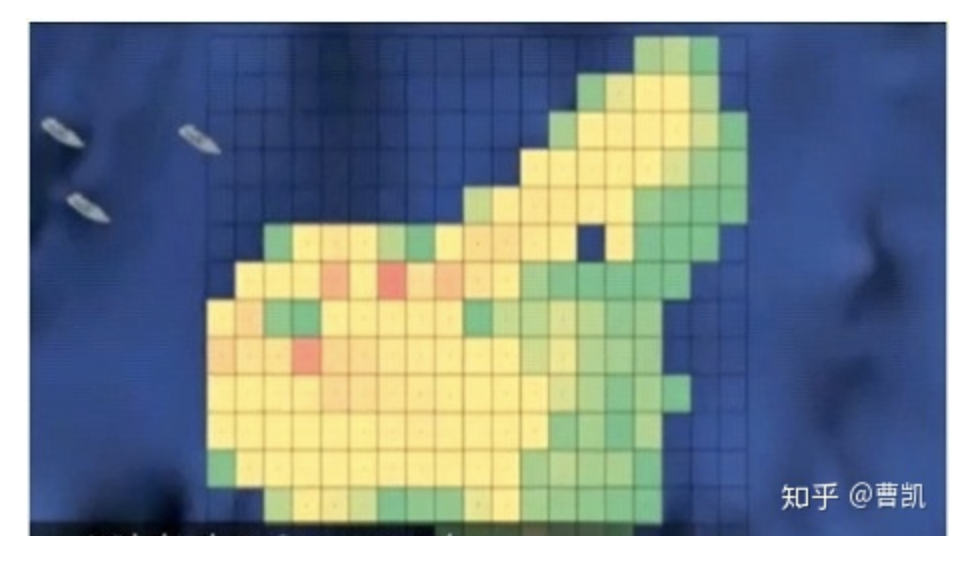
\includegraphics[width=.5\textwidth]{fig/Bayesian_Example_3.png}
\end{figure}
Craven又默默的写下了两行公式:
$$
p' = \frac{p(1-q)}{(1-p) + p(1-q)} = p\frac{1-q}{1-pq} < p
$$
$$
r' = r\frac{1}{1-pq} > r
$$

简单来讲:格子所在的海域是考虑到鱼雷冲击波,水流等因素后潜艇残骸可能散落的区域,$p$和$q$分别代表残骸散落到某个格子的概率以及在该格子内能够被找出来的概率(不是说在某个格子就一定能被找出来,这和海域深度有关系)。

到这,也许你会想:这有啥神奇的,计算概率嘛,整个统计学说的不就是概率么!别着急,再看:分母$1-pq$是大于分子$1-p$的, 所以$p'<p, r'>r$. 也就是说每次搜寻完一个格子后,残骸在这个格子里的概率$p'$就比之前$p$下降了;而同时,残骸在其它格子的概率就会上升。

所以,搜完一个格子后,全部区域都会重新洗牌,每次都会生成一个概率最大的格子,搜寻几次后某个格子的概率会特别大,美军只需要每次都驶向那个最大的,就能很快找到。

\section{朴素贝叶斯方法}
在实际应用贝叶斯法则的时候,通常会存在许多的条件,而不是单个条件。此时为了简化问题,我们有时候会做一个非常天真的假设,即\textbf{假设这些条件事件之间是相互独立的,这时候我们会得到朴素贝叶斯方法}。即:
\begin{align*}
P(A|X_1,X_2,\cdots,X_n) &= \frac{P(A,X_1,X_2,\cdots,X_n) }{P(X_1,X_2,\cdots,X_n)} \\
	&= \frac{P(A)P(X_1|A)P(X_2|A,X_1)\cdots P(X_n|A,X_1, X_2, \cdots, X_{n-1})}{P(X_1)P(X_2|X_1)P(X_3|X_1,X_2)\cdots P(X_n|X_1, X_2, \cdots, X_{n-1})} \\
	&= \frac{P(A)P(X_1|A)P(X_2|A)\cdots P(X_n|A)}{P(X_1)P(X_2)P(X_3)\cdots P(X_n)}
\end{align*}

\section{贝叶斯排序模型}
在对多条件下的后验概率进行展开时,除了运用朴素贝叶斯假设外,我们还可以使用另外一种迭代的方法。
$$
P(A|X_1,X_2,X_3) = P(((A|X_1)|X_2)|X_3)
$$

当存在更多的条件时,可以继续按照这个模式展开。以上展开表达式和各个条件事件的迭代顺序无关。下面是一个简单的证明:
\begin{align*}
P(A | X_1, X_2) &= \frac{P(A, X_1, X_2)}{P(X_1, X_2)} \\
P((A | X_1) | X_2) &= \frac{P(A, X_1| X_2)}{P(X_1|X_2)} = \frac{P(A, X_1, X_2)/P(X_2)}{P(X_1, X_2)/P(X_2)} = \frac{P(A, X_1, X_2)}{P(X_1, X_2)} \\
P((A | X_2) | X_1) &= \frac{P(A, X_1, X_2)}{P(X_1, X_2)} \\
\end{align*}

利用这种迭代展开式,我们可以构造一种贝叶斯排序模型,对诸多信息进行加工,生成主观概率。

\subsection{应用实例}
有两个同类别商品A和B,A有1个五星好评,B有5个五星好评和1个四星好评,那么你觉得这两个商品哪个更好一些呢?

实际上我们在对商品的诸多评论信息加工出一个对商品的整体评价时,使用的就是贝叶斯公式。进行如下定义:
\begin{itemize}
\setlength{\itemsep}{0pt}
\setlength{\parsep}{0pt}
\setlength{\parskip}{0pt}
    \item 事件 $X$:商品 $X$ 为非常棒的商品;
    \item 事件 $\bar{X}$:商品 $\bar{X}$ 为不是非常棒的商品;
\end{itemize}

那么,就有:
\begin{align*}
&P(A|5) = \frac{P(A)P(5|A)}{P(5|A)P(A) + P(5|\bar{A})P(\bar{A})} \\
&P(B|5,5,5,5,5,4) = P((((((B|5)|5)|5)|5)|5)|4)
\end{align*}

在没有任何信息的前提下,我们假设一个商品为非常棒的商品的概率为0.5,即:
$$
P(X) = 0.5
$$

并且我们假设,一个非常棒的商品获得各个星级的评价的概率分别如下,即我们假设非常棒的商品倾向于获得较高的评级。
\begin{align*}
P(1|X) &= 0.10; \\
P(2|X) &= 0.15; \\
P(3|X) &= 0.20; \\
P(4|X) &= 0.25; \\
P(5|X) &= 0.30; \\
\end{align*}

一个不是非常棒的商品获得各个星级的评价的概率分别如下,即我们假设不是非常棒的商品倾向于获得较低的评级。
\begin{align*}
P(1|\bar{X}) &= 0.30; \\
P(2|\bar{X}) &= 0.25; \\
P(3|\bar{X}) &= 0.20; \\
P(4|\bar{X}) &= 0.15; \\
P(5|\bar{X}) &= 0.10; \\
\end{align*}

迭代计算如下:
\begin{align*}
& P(A|5) = \frac{P(A)P(5|A)}{P(5|A)P(A) + P(5|\bar{A})P(\bar{A})} = \frac{0.5*0.3}{0.3*0.5+0.1*0.5} = 0.75 \\
& P(B|5) =  \frac{P(B)P(5|B)}{P(5|B)P(B) + P(5|\bar{B})P(\bar{B})} = \frac{0.5*0.3}{0.3*0.5+0.1*0.5} = 0.75 \\
& P(B|5|5) = \frac{0.9*0.3}{0.3*0.9+0.1*0.1} = 0.9 \\
& P(B|5|5|5) = \frac{0.75*0.3}{0.3*0.75+0.1*0.25} = 0.964286 \\
& P(B|5|5|5|5) = \cdots = 0.987805 \\
& P(B|5|5|5|5|5) = \cdots = 0.995902 \\
& P(B|5|5|5|5|5|4) = \cdots = 0.997537 \\
\end{align*}

于是我们得出结论:B商品更好。

%\printbibliography
\bibliography{../ref}
\bibliographystyle{IEEEtran}
\end{document}
